% Supports pdfLaTeX, XeLaTeX and LuaLaTeX on Overleaf.
\documentclass[12pt,a4paper,oneside]{report}
\usepackage{iftex}
\ifPDFTeX
  \usepackage[T1]{fontenc}
  \usepackage[utf8]{inputenc}
  \usepackage{tgtermes} % Times-compatible font for pdfLaTeX.
\else
  \usepackage{fontspec}
  % Optional: upload your own licensed Times New Roman files into fonts/.
  \IfFileExists{fonts/times.ttf}{%
    \setmainfont{times.ttf}[Path=fonts/,BoldFont=timesbd.ttf,
      ItalicFont=timesi.ttf,BoldItalicFont=timesbi.ttf]
  }{%
    \IfFontExistsTF{Times New Roman}{\setmainfont{Times New Roman}}%
      {\setmainfont{TeX Gyre Termes}}%
  }
\fi
\usepackage[left=29mm,right=22mm,top=22mm,bottom=22mm]{geometry}
\usepackage{graphicx}
\usepackage{setspace}
\usepackage{array,tabularx,booktabs}
\usepackage{enumitem}
\usepackage{caption}
\usepackage{float}
\usepackage{placeins}
\usepackage{titlesec}
\usepackage{tikz}
\usetikzlibrary{arrows.meta,positioning}
\usepackage[hidelinks,unicode]{hyperref}
\hypersetup{pdftitle={Secure Password Manager with Master-Key Encryption},
  pdfauthor={Siraj Riyaj Sayyad, Prathamesh Jayantkumar Sathe, Adesh Dattatray Dethe}}
\setstretch{1.25}
\setlength{\parindent}{0pt}
\setlength{\parskip}{5pt}
\setlength{\emergencystretch}{2em}
\setlist[itemize]{leftmargin=1.5em,itemsep=3pt,topsep=4pt,parsep=0pt}
\captionsetup{font=small,labelfont=bf}
\captionsetup[table]{position=top,skip=6pt}
\renewcommand{\arraystretch}{1.2}
\titleformat{\chapter}[hang]{\normalfont\Large\bfseries}{Chapter \thechapter:}{0.6em}{}
\titlespacing*{\chapter}{0pt}{0pt}{16pt}
\titleformat{\section}{\normalfont\large\bfseries}{\thesection}{0.6em}{}
\titleformat{\subsection}{\normalfont\normalsize\bfseries}{\thesubsection}{0.6em}{}
\setcounter{tocdepth}{1}
\raggedbottom

% Current preference: no printed page numbers and no page borders.
% Change false to true below to print Roman preliminary page numbers
% and Arabic numbers beginning with Chapter 1.
\newif\ifshowpagenumbers
\showpagenumbersfalse
\ifshowpagenumbers
  \pagestyle{plain}
\else
  \pagestyle{empty}
  \makeatletter\let\ps@plain\ps@empty\makeatother
\fi

\begin{document}

% ---- frontmatter ----
\begin{titlepage}
\centering
{\Large\bfseries Mini Project Phase I Report\par}
\vspace{8mm}
{\LARGE\bfseries Secure Password Manager with\\[2mm]Master-Key Encryption\par}
\vspace{8mm}
Submitted in partial fulfillment of the requirements for the award of\par
{\bfseries Final Year B.Tech. – Semester I\\Honors in Cyber Security\par}
\vspace{3mm}
{\bfseries CSE Hon-05B Mini Project\par}
\vspace{5mm}
Submitted to\par
{\bfseries Punyashlok Ahilyadevi Holkar Solapur University, Solapur\par}
\vspace{8mm}
{\bfseries Submitted by\par}
Mr. Siraj Riyaj Sayyad [Roll No. 70] [LY B]\\
Mr. Prathamesh Jayantkumar Sathe [Roll No. 68] [LY B]\\
Mr. Adesh Dattatray Dethe [Roll No. 46] [LY B]\par
{\bfseries Project Group No. B2\par}
\vspace{6mm}
Under the guidance of\par
{\bfseries Ms. A. S. Pathan\par}
\vspace{5mm}
\includegraphics[width=25mm]{images/college-logo.jpg}\par
\vfill
{\bfseries DEPARTMENT OF COMPUTER SCIENCE AND ENGINEERING\par}
{\large\bfseries SVERI'S COLLEGE OF ENGINEERING, PANDHARPUR\par}
\vspace{3mm}
Academic Year 2026–2027
\end{titlepage}

\clearpage\thispagestyle{empty}
\begin{center}
\includegraphics[width=25mm]{images/college-logo.jpg}\par
\vspace{4mm}
{\large\bfseries SVERI'S COLLEGE OF ENGINEERING, PANDHARPUR\par}
{\small Affiliated to Punyashlok Ahilyadevi Holkar Solapur University, Solapur\par}
\vspace{10mm}
{\LARGE\bfseries CERTIFICATE\par}
\end{center}
\vspace{6mm}
This is to certify that the Mini Project Phase I Report entitled
\begin{center}
{\large\bfseries Secure Password Manager with Master-Key Encryption\par}
\end{center}
has been successfully submitted by
\begin{center}
Mr. Siraj Riyaj Sayyad [Roll No. 70] [LY B]\\
Mr. Prathamesh Jayantkumar Sathe [Roll No. 68] [LY B]\\
Mr. Adesh Dattatray Dethe [Roll No. 46] [LY B]
\end{center}
in partial fulfillment of the requirements for Final Year B.Tech. – Semester I
of Honors in Cyber Security for the subject CSE Hon-05B Mini Project,
as per the curriculum prescribed by Punyashlok Ahilyadevi Holkar Solapur
University, Solapur, during the Academic Year 2026–2027.

\vspace{15mm}
\noindent\begin{minipage}[t]{0.49\linewidth}
\textbf{Ms. A. S. Pathan}\\Project Guide
\end{minipage}\hfill
\begin{minipage}[t]{0.45\linewidth}
\textbf{Dr. Vanita Jadhav}\\Head of Department CSE
\end{minipage}
\vspace{15mm}
\begin{center}\textbf{Dr. B. P. Ronge}\\Principal\end{center}
\vspace{8mm}
Place: Pandharpur\hfill Date: \rule{32mm}{0.4pt}

\clearpage
\pagenumbering{roman}
\chapter*{Abstract}
\addcontentsline{toc}{chapter}{Abstract}
With the increasing use of web applications, online banking, cloud platforms, social media, educational portals, and software services, users are required to manage a large number of usernames and passwords. Reusing passwords or storing credentials in ordinary notes and unprotected files creates a significant security risk. The proposed Secure Password Manager with Master-Key Encryption provides a centralized and protected vault for storing credentials. The system uses a master password as the primary authentication secret and derives a cryptographic key from it using a salt and a suitable key-derivation process. Sensitive credential information is encrypted before storage and decrypted only after successful authentication. The proposed system also provides password generation, password-strength checking, credential search, add, view, update, and delete operations, together with secure logout and session protection. AES-256 or another strong authenticated encryption mechanism can be used for protecting stored data, while password hashing is used where verification rather than recovery is required. The project aims to demonstrate practical application of cryptography, authentication, access control, and secure software design in a realistic B.Tech CSE mini-project.

\clearpage
\tableofcontents
\clearpage

\clearpage
\pagenumbering{arabic}

% ---- chapters/chapter1 ----
\chapter{Project Overview}

\section{Title of the Mini Project}

Secure Password Manager with Master-Key Encryption
\section{Introduction}

\subsection{Background}

A password manager is a security application designed to reduce the difficulty of remembering many unique credentials while improving the protection of those credentials. Instead of asking a user to remember every individual password, the application protects a secure collection of credentials using one master password. The master password is not treated as an ordinary application password; it is used to authenticate the user and derive or unlock the key material required to protect the vault.

In the proposed project, each credential record may contain a service name, website or application identifier, username, password, and optional notes. These records are treated as sensitive data. The application encrypts sensitive fields before they are persisted in the vault. A random salt is stored with the vault parameters, while the master password itself is never stored in plaintext. This design separates authentication information from recoverable credential data and demonstrates the principle of least exposure.

\subsection{Current Scenario}

Users commonly maintain credentials across dozens of websites and applications. Many users still reuse a familiar password, save passwords in browser notes or text files, or keep credentials in unencrypted documents. Although browsers and commercial password managers provide convenient storage, users may not understand how credentials are protected, how a master secret is handled, or what happens when a device is shared. A mini-project implementation is useful because it makes the underlying security workflow visible and provides a controlled environment for learning.

Modern password-management systems generally combine strong authentication, cryptographic protection, secure local storage, password generation, and session controls. The proposed project follows the same fundamental security direction while intentionally keeping the scope manageable for a Phase I academic project.

\subsection{Existing Challenges}

\begin{itemize}
\item Users often reuse weak or predictable passwords across multiple services.
\item Credentials stored in plain text or ordinary documents can be exposed if the device is compromised.
\item Remembering many unique passwords creates usability problems and encourages insecure shortcuts.
\item A password database itself becomes a high-value target and therefore requires encryption and controlled access.
\item Weak master-password handling can undermine otherwise strong encryption.
\item Poor session management may leave an unlocked vault accessible to another person using the same device.
\end{itemize}

\subsection{Motivation}

The motivation for this project is to create a practical demonstration of how cryptographic protection can be integrated into a usable application. The project connects concepts studied in cybersecurity and computer science—hashing, salts, key derivation, symmetric encryption, authentication, access control, secure storage, and session management—into one coherent system.

\subsection{Overview of Proposed Work}

The proposed system begins with secure master-password setup. A salt and key-derivation mechanism are used to produce key material from the master password. After authentication, the user can create and manage credential records. Sensitive values are encrypted before storage and decrypted only for authorized operations. A password generator creates strong random passwords, while a strength checker gives feedback before a password is saved. The application also provides search, edit, delete, timeout, and logout functions.

\section{Need for the Project (Relevance / Significance)}

Industrial Need: Centralized credential storage reduces password reuse and provides a controlled mechanism for protecting sensitive authentication data.

Social Need: Better password practices reduce the likelihood of account takeover caused by reused, weak, or exposed passwords.

Academic Need: The project gives practical exposure to encryption, password hashing, key derivation, authentication, secure database design, and security testing.

Technical Significance: It demonstrates the difference between storing a password for verification and encrypting data that must later be recovered by an authorized user.


% ---- chapters/chapter2 ----
\chapter{Literature Study}

\section{Literature Review}

\begin{itemize}
\item NIST SP 800-63B discusses digital identity and authenticator management, emphasizing secure handling of memorized secrets and resistance to common authentication attacks. The present project applies these principles by treating the master password as a high-value authentication secret and avoiding plaintext storage. (NIST Digital Identity Guidelines)
\item OWASP guidance on password storage recommends modern password hashing algorithms, unique salts, and appropriate work factors for passwords that need verification. The project uses this principle for master-password verification where direct password recovery is not required. (OWASP Password Storage Guidance)
\item FIPS 197 specifies the Advanced Encryption Standard (AES), a widely used symmetric encryption standard. AES-256 is considered for encrypting the credential vault because the stored passwords must remain recoverable for authorized use. (NIST FIPS 197)
\item RFC 8018 describes password-based cryptography and the use of a password-based key derivation function such as PBKDF2 with a salt and iteration count. This provides a useful foundation for deriving vault key material from a human-generated master password. (RFC 8018)
\item NIST SP 800-57 provides guidance on cryptographic key management. It emphasizes lifecycle management, protection, access control, and appropriate handling of cryptographic keys. The project uses these concepts to keep derived key material within the protected session and to avoid exposing it as normal application data. (NIST SP 800-57)
\item Bonneau et al. studied the difficulty of achieving both usable and secure authentication systems. Their work highlights the tension between strong security and user convenience. The proposed password manager addresses this tension by reducing the number of passwords the user must remember while encouraging unique generated credentials. (Bonneau et al., The Quest to Replace Passwords)
\item Florêncio and Herley investigated password habits and showed that users face a large management burden when they maintain many accounts. Their findings support the need for tools that reduce password reuse and the cognitive load associated with multiple credentials. (Florêncio and Herley, Password Management)
\item Gaw and Felten examined how users manage passwords and observed practical behaviors such as reuse and informal storage. The proposed system provides a safer alternative by giving users a dedicated encrypted vault and generation tools. (Gaw and Felten, Password Management Practices)
\item Stobert and Biddle studied password management behavior and the role of password managers in improving security. Their work supports the usability value of automated credential storage and retrieval. The project incorporates these functions through a simple vault interface and search capability. (Stobert and Biddle, Password Manager Usability)
\item Ur et al. examined users’ perceptions of password managers and found that trust and understanding influence adoption. The proposed project therefore keeps the security workflow visible and explains the role of the master password, encryption, and session protection. (Ur et al., Password Manager Perceptions)
\item Li et al. analyzed password-manager security and identified risks associated with implementation errors, credential exposure, and insecure integration. This motivates the project’s focus on a minimal attack surface and explicit separation of authentication, encryption, and storage modules. (Li et al., Password Manager Security)
\item Silver et al. evaluated password-manager usability and security characteristics and demonstrated that automation can encourage stronger password practices. The proposed generator and strength checker are included for the same purpose. (Silver et al., Password Manager Evaluation)
\item NIST SP 800-132 discusses password-based key derivation and the use of salts in deriving cryptographic keys from passwords. This supports the project’s design of deriving a vault key from the master password rather than storing the key directly. (NIST SP 800-132)
\item Kaliski’s work on PKCS specifications provides background for password-based encryption and key-derivation mechanisms. These standards are relevant to implementing interoperable and well-understood cryptographic workflows. (Kaliski, PKCS Specifications)
\item The use of authenticated encryption has become important because confidentiality alone does not guarantee that stored ciphertext has not been modified. The project therefore considers an authenticated encryption mode such as AES-GCM for practical implementation, where available. (Authenticated Encryption Literature)
\item Salted password hashing is distinct from reversible encryption. Hashing is appropriate when the system only needs to verify a password, whereas encryption is required when the application must later recover a stored credential. This distinction forms a key design principle of the proposed system. (Password Hashing and Encryption Principles)
\item Key-derivation functions slow down large-scale password guessing by making each password trial computationally more expensive. The project uses a configurable work factor and salt to strengthen the derived master key against offline guessing. (Key Derivation Research)
\item Secure random number generation is necessary for salts, initialization vectors or nonces, and generated passwords. Predictable random values can weaken otherwise strong cryptographic algorithms. The project therefore treats randomness as a security-critical service. (Cryptographic Randomness Principles)
\item Least-privilege access control limits which application functions can access sensitive credential data. The proposed architecture restricts vault access to authenticated sessions and keeps credential operations behind the authentication layer. (Access Control Literature)
\item Secure session management reduces the time during which an unlocked vault remains exposed. Timeout and explicit logout are therefore included in the project to reduce risk when a device is left unattended. (Session Security Literature)
\item Usable security research shows that complicated security mechanisms may be ignored when they create excessive user effort. The project therefore combines strong protection with straightforward add, search, edit, and delete operations. (Usable Security Research)
\item Threat modeling methods such as STRIDE can be used to identify threats against authentication, stored data, and application interfaces. For this project, threat analysis is focused on unauthorized vault access, credential disclosure, tampering, and session misuse. (Threat Modeling Literature)
\item Secure software-development practices recommend validating input, minimizing sensitive data lifetime, avoiding unnecessary logging of secrets, and separating security-critical components. These principles guide the proposed credential-management modules. (Secure Software Development Literature)
\item Database-security research emphasizes access control, encryption at rest, and careful treatment of sensitive columns. The project applies these principles by storing only encrypted credential values and restricting access through the authenticated application session. (Database Security Literature)
\item Client-side storage must be treated carefully because a local attacker may inspect application files. The project therefore avoids storing the master password in configuration files and treats the vault database as encrypted data rather than trusted plaintext storage. (Client-Side Storage Security)
\item Password-strength estimation techniques can identify short, predictable, or commonly patterned passwords. The project uses a practical strength checker to provide immediate feedback before a generated or user-entered password is saved. (Password Strength Research)
\item Password generators can create unique random passwords with configurable length and character classes. Such automation reduces the temptation to reuse familiar passwords across multiple services. (Password Generation Research)
\item Cryptographic key separation recommends using distinct keys or derived subkeys for different purposes where appropriate. The project can derive vault-encryption material independently from authentication-verification material so that compromise of one representation does not directly reveal another. (Cryptographic Key Separation)
\item Backup and recovery research highlights the importance of protecting encrypted backups and recovery information. The project keeps recovery mechanisms out of the Phase I core unless they can be designed without weakening the master-key security model. (Secure Backup Research)
\item Recent password-manager research continues to emphasize implementation correctness, secure defaults, and transparent security boundaries. The proposed project addresses these themes through a focused architecture, limited scope, and explicit security requirements. (Recent Password Manager Research)
\end{itemize}

\section{Research Gap}

Existing password managers demonstrate that centralized credential storage can improve usability and reduce password reuse, but they also introduce a new high-value target: the password vault itself. Security therefore depends not only on the strength of individual stored passwords but also on the protection of the master secret, key derivation process, encryption parameters, session handling, and application storage.

A common limitation in simplified student implementations is that they store credentials directly in databases or use a single hash as if it were reversible encryption. Such designs do not adequately distinguish authentication verification from confidential data recovery. Another limitation is insufficient attention to salt management, secure random values, logout behavior, and the lifetime of decrypted data.

\begin{itemize}
\item Many basic credential-storage applications do not clearly separate password hashing from reversible vault encryption.
\item Some implementations use weak or fixed keys rather than deriving key material from a protected master secret.
\item Usability features such as generation, search, update, and strength feedback are sometimes implemented without a complete security model.
\item Session protection and secure logout are frequently treated as interface features rather than security controls.
\item Backup, local-storage, and access-control considerations are often outside the initial design.
\end{itemize}

The proposed project addresses these gaps through a focused master-key model: a master password authenticates the user, a salt and key-derivation process produce cryptographic key material, sensitive credentials are encrypted before storage, and credential operations are available only inside an authenticated session. The design remains intentionally small enough for a B.Tech Phase I project while providing a technically meaningful security foundation.


% ---- chapters/chapter3 ----
\chapter{Problem Definition}

\section{Problem Statement}

Users are required to maintain many accounts across websites, applications, cloud services, educational systems, banking platforms, and communication tools. Remembering separate strong passwords for every service is difficult, so users often reuse passwords, select predictable patterns, or store credentials in insecure locations. If a stored credential file is exposed, an attacker may obtain multiple accounts at once. The problem is therefore to design a secure and usable password manager that stores credentials centrally while protecting the vault through a master-key-based encryption mechanism.

\section{Objectives of the Project}

\begin{itemize}
\item Securely store usernames, passwords, service names, and optional notes in a protected credential vault.
\item Use a master password for authentication and derive cryptographic key material using a salt and suitable key-derivation process.
\item Encrypt sensitive credential data before persistence and decrypt it only after successful authentication.
\item Provide a secure password generator for creating unique and difficult-to-guess passwords.
\item Provide password-strength checking and useful feedback before credentials are stored.
\item Allow authorized users to add, view, update, delete, and search credential records.
\item Protect sensitive data from unauthorized access through access control and secure session handling.
\item Provide explicit logout and automatic session timeout to reduce exposure on unattended devices.
\item Demonstrate practical application of cryptography and secure software-development principles.
\end{itemize}

\section{Scope of the Project}

Included: master-password setup and authentication; key derivation; encrypted credential storage; add, view, edit, delete, and search operations; password generation; password-strength checking; basic session timeout and logout; local database or secure storage; security testing of the core workflow.

Excluded from Phase I: enterprise identity federation, biometric authentication, multi-device synchronization, browser extensions, cloud-based sharing, emergency recovery services, hardware security modules, and commercial-scale deployment. These features may be evaluated as future enhancements after the core vault is validated.


% ---- chapters/chapter4 ----
\chapter{Proposed Work}

\section{Proposed Methodology}

\subsection{Overall Workflow}

\begin{itemize}
\item User registration or first-time vault setup.
\item Master password creation with strength validation and confirmation.
\item Generation of a random salt and derivation of master-key material using a suitable KDF.
\item Secure authentication by verifying the master password or its protected verifier.
\item Opening the encrypted credential vault only after successful authentication.
\item Adding credential information such as service name, username, password, URL, and optional notes.
\item Encrypting sensitive fields using a strong symmetric encryption mechanism before storage.
\item Retrieving the encrypted record from the vault and decrypting it only inside an authorized session.
\item Editing or deleting records and securely updating the encrypted database entry.
\item Searching records without exposing the stored plaintext outside the application interface.
\item Generating strong random passwords and evaluating password strength.
\item Locking or logging out the session after inactivity or explicit user action.
\end{itemize}

\subsection{System Design}

The proposed system is divided into independent security and functional modules. The Authentication Module manages master-password setup and verification. The Key-Derivation Module converts the master password into key material using a random salt and an appropriate work factor. The Encryption Module protects credential fields. The Credential Vault manages encrypted records and database operations. The Password Utility Module provides password generation and strength feedback. Finally, the Session Security Module controls timeout, lock, and logout behavior.

\subsection{Cryptographic Design}

A practical implementation may use AES-256 in an authenticated-encryption mode such as AES-GCM. A fresh nonce/initialization value is generated for each encryption operation and stored with the ciphertext as non-secret metadata. The master password is processed through a password-based key-derivation function such as PBKDF2, Argon2id, or scrypt, depending on the selected implementation environment. The salt is stored with the vault parameters because it does not need to remain secret. The master password itself is never stored in plaintext.

\subsection{Data Model}

A credential record can contain: Credential ID, Service Name, Website/URL, Username, Encrypted Password, Encrypted Notes, Created Date, Updated Date, and optional category information. Only non-sensitive metadata should remain directly readable. Password and private notes should remain encrypted at rest.

\subsection{Data Collection and Preparation}

The project does not require a machine-learning dataset. Instead, test data consists of synthetic credential records created for functional and security testing. Test cases include short and strong master passwords, multiple credential records, duplicate service names, long passwords, special characters, empty fields, invalid input, and repeated authentication attempts. No real banking or personal credentials should be used during development.

\subsection{Testing}

\begin{itemize}
\item Verify successful vault creation using a valid master password.
\item Verify rejection of incorrect master-password attempts.
\item Verify that plaintext passwords are not present in the stored database.
\item Verify encryption and decryption of credential records.
\item Verify that each encryption operation uses fresh nonce/IV values as required by the selected algorithm.
\item Verify add, view, edit, delete, and search functions.
\item Verify generated passwords meet configured length and character requirements.
\item Verify password-strength feedback for weak, medium, and strong examples.
\item Verify automatic locking after inactivity and successful logout.
\item Verify that unauthorized screens or database operations cannot access decrypted credentials.
\end{itemize}

\subsection{Performance and Security Evaluation}

The system can be evaluated using functional correctness, encryption/decryption time, vault-opening time, password-generation time, search response time, memory usage, and behavior as the number of credential records increases. Security evaluation focuses on plaintext exposure, incorrect authentication handling, predictable cryptographic values, improper session persistence, and accidental logging of secrets. The goal is not to claim commercial-grade security but to demonstrate that the implemented controls work consistently under the defined Phase I scope.

\section{System Architecture}
\begin{figure}[H]
\centering
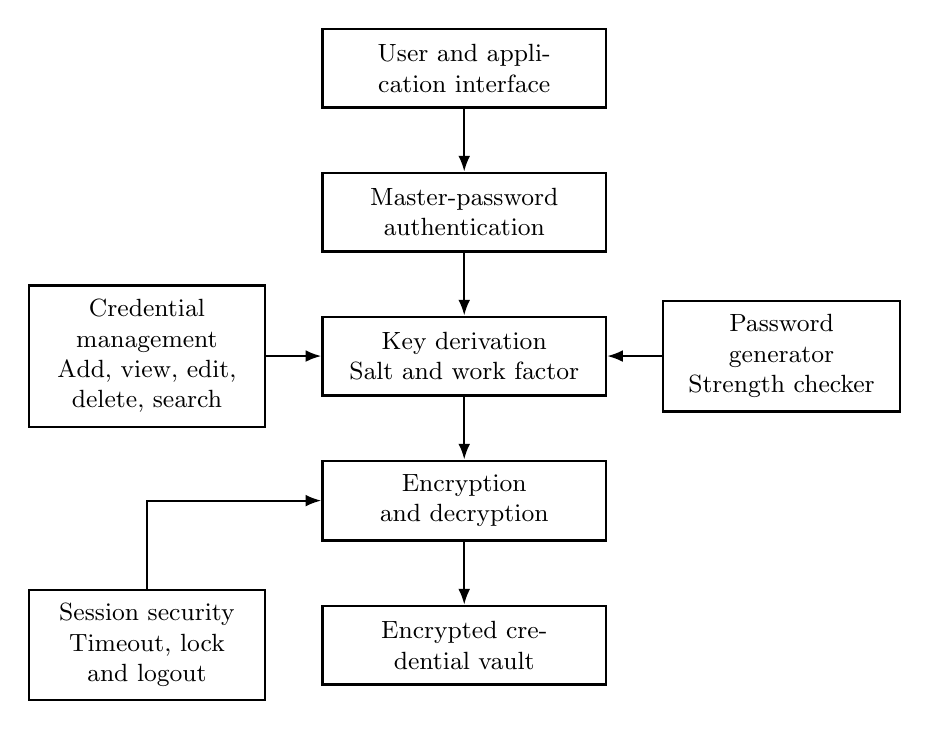
\begin{tikzpicture}[
  box/.style={draw,thick,align=center,text width=3.25cm,
    minimum height=1cm,inner sep=5pt,font=\small},
  side/.style={box,text width=2.65cm},
  flow/.style={-{Latex[length=2mm]},thick},
  node distance=8mm]
\node[box] (user) {User and application interface};
\node[box,below=of user] (auth) {Master-password authentication};
\node[box,below=of auth] (kdf) {Key derivation\\Salt and work factor};
\node[box,below=of kdf] (crypto) {Encryption and decryption};
\node[box,below=of crypto] (vault) {Encrypted credential vault};
\node[side,left=7mm of kdf] (manage) {Credential management\\Add, view, edit, delete, search};
\node[side,right=7mm of kdf] (utility) {Password generator\\Strength checker};
\node[side,left=7mm of vault] (session) {Session security\\Timeout, lock and logout};
\draw[flow] (user)--(auth);
\draw[flow] (auth)--(kdf);
\draw[flow] (kdf)--(crypto);
\draw[flow] (crypto)--(vault);
\draw[flow] (manage)--(kdf);
\draw[flow] (utility)--(kdf);
\draw[flow] (session.north)|-(crypto.west);
\end{tikzpicture}
\caption{Secure password manager system architecture}
\label{fig:architecture}
\end{figure}
The User interacts with the application through the authentication layer. After the master password is successfully verified, the key-derivation module produces the session key material required to unlock the vault. The encryption/decryption module then protects credential data as it moves between the application and the database. Credential Management provides the normal add, view, edit, delete, and search operations, while the Password Generator and Strength Checker support safer password creation. Session Security ensures that the unlocked vault is not left available indefinitely. This separation of responsibilities makes the system easier to test and reduces the chance that a user-interface component directly handles persistent plaintext credentials.

\section{Hardware Requirements}
\begin{table}[H]
\centering
\caption{Hardware requirements}
\label{tab:hardware}
\small
\begin{tabularx}{\linewidth}{@{}p{.21\linewidth}p{.35\linewidth}X@{}}
\toprule
\textbf{Component} & \textbf{Specification} & \textbf{Function} \\
\midrule
Computer System & Intel i3/i5 or higher, 4 GB+ RAM & Development and testing platform \\
Storage & 250 GB HDD/SSD or higher & Application, database, and test-data storage \\
Display & Standard HD display & Application interface and testing \\
Network & Internet connection when required & Package installation and optional updates \\
\bottomrule
\end{tabularx}
\end{table}
The hardware requirements describe the proposed development and testing platform. Storage supports the application and synthetic test records; internet access is needed for package installation and optional updates.
\section{Software Requirements}

\begin{itemize}
\item Programming Language: Python 3.x or another suitable secure application language.
\item IDE: Visual Studio Code / PyCharm.
\item Cryptography Library: A maintained library supporting AES and secure random generation.
\item Key-Derivation / Hashing: PBKDF2, Argon2id, or scrypt as supported by the selected implementation.
\item Database/Storage: SQLite or another lightweight local database with protected credential fields.
\item Operating System: Windows 10/11 or Linux.
\item Testing Tools: Unit-testing framework and manual security test cases.
\end{itemize}

\subsection{Security Requirements}

\begin{itemize}
\item Never store the master password in plaintext.
\item Never write decrypted passwords to application logs.
\item Use a unique salt for each vault.
\item Use a unique nonce/IV for each encryption operation when required by the selected mode.
\item Clear or minimize sensitive data held in memory after use where practical.
\item Lock the vault after a configurable period of inactivity.
\end{itemize}


% ---- chapters/chapter5 ----
\chapter{Project Planning}

\section{Working Steps / Activity Plan}

\begin{itemize}
\item Requirement analysis and study of password-management and cryptographic concepts.
\item Literature review and identification of security requirements.
\item Design of system architecture, database schema, and module interfaces.
\item Design of master-password authentication and key-derivation workflow.
\item Development of encryption/decryption and secure storage modules.
\item Development of credential-management interface and CRUD operations.
\item Development of password generator and password-strength checker.
\item Implementation of session timeout, vault lock, and secure logout.
\item Integration, functional testing, and security-focused testing.
\item Documentation, review, corrections, and final report preparation.
\end{itemize}

\section{Expected Date of Completion of Work}
\begin{table}[H]
\centering
\caption{Proposed activity schedule}
\label{tab:schedule}
\small
\begin{tabularx}{\linewidth}{@{}X p{.30\linewidth}@{}}
\toprule
\textbf{Activity} & \textbf{Duration} \\
\midrule
Project Start & June 2026 \\
Requirement Analysis \& Literature Review & June–July 2026 \\
Architecture \& Security Design & July 2026 \\
Core Development & July–August 2026 \\
Testing \& Validation & August–September 2026 \\
Documentation \& Review & September 2026 \\
Expected Completion & September 2026 \\
\bottomrule
\end{tabularx}
\end{table}
The schedule records the June–September 2026 plan provided in the source report. It describes the intended sequence of activities and does not confirm actual completion.
\section{Approximate Expenditure}
\begin{table}[H]
\centering
\caption{Estimated project expenditure}
\label{tab:budget}
\small
\begin{tabularx}{\linewidth}{@{}p{.09\linewidth}X p{.14\linewidth}p{.19\linewidth}@{}}
\toprule
\textbf{Sr. No.} & \textbf{Item} & \textbf{Quantity} & \textbf{Approx. Cost (Rs.)} \\
\midrule
1 & Software licenses (if any) & -- & 500 \\
2 & Internet/Cloud usage & -- & 500 \\
3 & Printing \& Documentation & -- & 1,000 \\
4 & Miscellaneous & -- & 500 \\
 & Total &  & 2,500 \\
\bottomrule
\end{tabularx}
\end{table}
The estimated expenditure totals Rs. 2,500. These values are the original budget estimates and are not records of actual purchases. Quantities were not specified in the source report.
\section{Available Facilities}

\begin{itemize}
\item Computer laboratory with internet access.
\item Development systems capable of running the selected programming language and database.
\item Visual Studio Code / PyCharm development environment.
\item Cryptography and database libraries available through standard package managers.
\item Faculty guidance from the Department of Computer Science and Engineering.
\item Laboratory resources for functional and security testing.
\end{itemize}

\subsection{Implementation Plan and Risk Control}

The project will be developed incrementally so that security-critical components are tested before user-interface integration. First, the team will validate the master-password and key-derivation workflow. Next, encrypted storage and retrieval will be implemented and tested using synthetic records. Credential-management operations will then be added, followed by password-generation, strength checking, and session security. This order reduces the risk of building interface features around an insecure storage model.

Major project risks include incorrect cryptographic API usage, accidental plaintext logging, weak password handling, and loss of access to a test vault. These risks will be reduced by using established libraries, avoiding custom cryptographic algorithms, maintaining test-only credentials, reviewing sensitive code separately, and keeping controlled development backups of encrypted test data.

\subsection{Milestones}

\begin{itemize}
\item Milestone 1: Requirements, literature review, and threat identification completed.
\item Milestone 2: Architecture and data model approved.
\item Milestone 3: Master-key derivation and encrypted vault implemented.
\item Milestone 4: Credential-management and password utilities integrated.
\item Milestone 5: Security testing and corrections completed.
\item Milestone 6: Final documentation and demonstration prepared.
\end{itemize}


% ---- chapters/chapter6 ----
\chapter{Expected Results}

\section{Expected Outcome}

\begin{itemize}
\item A functional secure credential vault for storing multiple service accounts.
\item Master-password-based authentication with derived cryptographic key material.
\item Encrypted storage of sensitive credential information.
\item Working add, view, edit, delete, and search operations for authorized users.
\item Password generation and strength-checking functionality.
\item Secure logout and session timeout to reduce exposure from unattended sessions.
\item Test evidence demonstrating that plaintext passwords are not intentionally stored in the database.
\end{itemize}

\section{Innovation / Novelty}

\begin{itemize}
\item Combines usability-oriented password management with a clearly defined master-key security model.
\item Separates password verification concepts from reversible encryption of recoverable credentials.
\item Uses salt and key derivation instead of a fixed encryption key embedded in application code.
\item Includes password generation and strength feedback as part of the security workflow.
\item Treats session locking and logout as security controls rather than only interface functions.
\end{itemize}

\section{Applications}

\begin{itemize}
\item Personal credential management.
\item Small-office and educational demonstrations of secure storage.
\item Cybersecurity laboratory exercises.
\item Demonstration of encryption and key-derivation concepts.
\item Prototype foundation for future browser, mobile, or cloud-integrated password-management systems.
\end{itemize}

\section{Advantages}

\begin{itemize}
\item Reduces password reuse by helping users maintain unique credentials.
\item Protects stored credentials through encryption.
\item Provides centralized and searchable credential management.
\item Automates creation of stronger passwords.
\item Provides a manageable architecture for a B.Tech CSE project.
\item Supports practical learning of cryptography and secure application development.
\end{itemize}

\section{Limitations}

\begin{itemize}
\item The security of the vault depends strongly on the secrecy and strength of the master password.
\item A forgotten master password may make encrypted credentials unrecoverable if no secure recovery mechanism is implemented.
\item The Phase I version is intended for controlled academic use and is not a commercial password manager.
\item The project does not include enterprise identity federation, browser extensions, or multi-device synchronization.
\item Security can still be affected by a compromised operating system, malware, or a maliciously modified application.
\item Cryptographic implementation must rely on trusted libraries and correct API usage; custom cryptography is outside the project scope.
\end{itemize}

\section{Future Scope}

\begin{itemize}
\item Add secure browser-extension integration for automatic credential filling.
\item Provide optional mobile and desktop clients using the same security model.
\item Introduce carefully designed encrypted synchronization across trusted devices.
\item Support secure import/export with explicit user confirmation and protected export files.
\item Add stronger device-bound protections or hardware-backed key storage where supported.
\item Provide security auditing, vault health checks, and detection of reused or weak passwords.
\item Evaluate modern memory-hard key-derivation methods and authenticated encryption implementations.
\item Add controlled recovery mechanisms without storing a plaintext master password or unrestricted recovery key.
\end{itemize}

\section{Environmental and Social Impact}

The project supports safer digital participation by encouraging unique passwords and reducing unsafe credential storage practices. Better credential hygiene can lower the risk of account compromise and associated disruption. The application is software-based and requires no dedicated hardware beyond an ordinary computer, so the direct environmental footprint is small. By centralizing security controls in software, the project also supports responsible digital-security education and awareness.

The social impact is mainly preventive: users learn that convenience and security can be combined when sensitive information is protected by strong authentication, encryption, and controlled access. The project can also be used as an academic demonstration for secure software-development principles.


% ---- chapters/chapter7 ----
\chapter{Conclusion}

The proposed Secure Password Manager with Master-Key Encryption provides a practical approach to the problem of managing multiple credentials without relying on insecure plaintext storage or repeated passwords. The system uses a master password as the primary authentication secret and derives cryptographic key material through a salted key-derivation process. Sensitive credentials are encrypted before being stored in the secure vault and are made available only after successful authentication.

The project combines secure credential storage with practical features such as password generation, strength checking, credential search, add, view, edit, delete, session timeout, and logout. These functions demonstrate how security controls can be integrated into a usable application instead of being treated as isolated cryptographic operations.

A major technical objective of the project is to clearly distinguish password hashing from encryption. A password that only needs verification should be protected with a suitable password-hashing or key-derivation mechanism, while credentials that the user must later retrieve require reversible encryption. Salt management, unique nonces or initialization values, access control, and session protection further strengthen the design.

Within the scope of a B.Tech CSE Mini Project Phase I, the proposed system provides a realistic foundation for studying confidentiality, authentication, key management, and secure software development. Future versions can extend the design to synchronization, browser integration, device-bound security, and additional recovery mechanisms. Overall, the project demonstrates how a carefully designed master-key model can improve credential security while maintaining practical usability.

The project also establishes a clear security boundary: the master password unlocks access, the derived key protects the vault, and the application exposes credentials only through authorized operations. This layered approach provides a practical example of how security, usability, and maintainability can be considered together during software design.


% ---- references ----
\clearpage
\phantomsection
\addcontentsline{toc}{chapter}{References}
\renewcommand{\bibname}{References}
\begin{thebibliography}{99}
\small
\setlength{\itemsep}{4pt}
\bibitem{ref1} National Institute of Standards and Technology, “Digital Identity Guidelines: Authentication and Lifecycle Management,” NIST SP 800-63B, latest revision.

\bibitem{ref2} National Institute of Standards and Technology, “Advanced Encryption Standard (AES),” FIPS PUB 197, 2001.

\bibitem{ref3} National Institute of Standards and Technology, “Recommendation for Password-Based Key Derivation,” NIST SP 800-132, 2010.

\bibitem{ref4} National Institute of Standards and Technology, “Recommendation for Key Management,” NIST SP 800-57 Part 1, Revision 5.

\bibitem{ref5} M. Moriarty, B. Kaliski, and J. Jonsson, “PKCS \#5: Password-Based Cryptography Specification Version 2.1,” RFC 8018, IETF, 2017.

\bibitem{ref6} OWASP Foundation, “Password Storage Cheat Sheet,” OWASP Cheat Sheets, security guidance for password hashing and storage.

\bibitem{ref7} OWASP Foundation, “Authentication Cheat Sheet,” OWASP Cheat Sheets, guidance on authentication controls.

\bibitem{ref8} C. Bonneau, C. Herley, P. C. van Oorschot, and F. Stajano, “The Quest to Replace Passwords: A Framework for Comparative Evaluation of Web Authentication Schemes,” IEEE Symposium on Security and Privacy, 2012.

\bibitem{ref9} H. M. Gaw and A. S. Felten, “Password Management Strategies for Online Accounts,” ACM-related password-management research, 2006.

\bibitem{ref10} M. Florêncio and C. Herley, “A Large-Scale Study of Web Password Habits,” Proceedings of the International World Wide Web Conference, 2007.

\bibitem{ref11} A. Stobert and R. Biddle, “The Password Is Dead! Long Live the Password: A Qualitative Study of Password Practices,” CHI-related password research.

\bibitem{ref12} E. Ur, F. N. Al-Ameen, A. B. K. et al., research on user perceptions, adoption, and usability of password managers.

\bibitem{ref13} Z. Li, W. He, D. Akhawe, and D. Song, research on password-manager security and credential exposure risks.

\bibitem{ref14} B. Ross, C. Jackson, N. Miyake, D. Boneh, and M. Mitchell, “Stronger Password Authentication Using Browser-Based Password Managers,” Web security research.

\bibitem{ref15} J. Bonneau and C. Preibusch, research on the economics and usability of online password systems.

\bibitem{ref16} A. Adams and M. A. Sasse, “Users Are Not the Enemy: Why Users Compromise Computer Security Mechanisms and How to Take a Constructive Approach,” Communications of the ACM, 1999.

\bibitem{ref17} E. W. Felten and related usable-security research on human factors in authentication and password management.

\bibitem{ref18} A. Menezes, P. van Oorschot, and S. Vanstone, “Handbook of Applied Cryptography,” CRC Press, 1996.

\bibitem{ref19} W. Stallings, “Cryptography and Network Security: Principles and Practice,” Pearson, reference text on symmetric encryption, authentication, and key management.

\bibitem{ref20} NIST, “Recommendation for Random Number Generation Using Deterministic Random Bit Generators,” NIST SP 800-90A, Rev. 1.

\bibitem{ref21} OWASP Foundation, “Cryptographic Storage Cheat Sheet,” guidance on encryption, key management, and secure storage of sensitive information.

\bibitem{ref22} P. Rogaway, “Authenticated-Encryption with Associated Data,” cryptographic literature on confidentiality and integrity.

\bibitem{ref23} M. Bellare and C. Namprempre, research on authenticated encryption and the relationship between confidentiality and integrity.

\bibitem{ref24} E. Barker, “Recommendation for Key-Derivation Methods in Key-Establishment Schemes,” NIST SP 800-56C.

\bibitem{ref25} NIST, “Security and Privacy Controls for Information Systems and Organizations,” NIST SP 800-53, reference for access control and system protection.

\bibitem{ref26} OWASP Foundation, “Logging Cheat Sheet,” guidance for avoiding sensitive information exposure through application logs.

\end{thebibliography}


% ---- submission ----
\FloatBarrier
\section*{Submission and Signatures}
Date of Mini Project Phase I submission: \rule{55mm}{0.4pt}

\vspace{6mm}
\textbf{Names, roll numbers and signatures of the students}

Mr. Siraj Riyaj Sayyad [Roll No. 70]\\Signature: \rule{65mm}{0.4pt}

Mr. Prathamesh Jayantkumar Sathe [Roll No. 68]\\Signature: \rule{65mm}{0.4pt}

Mr. Adesh Dattatray Dethe [Roll No. 46]\\Signature: \rule{65mm}{0.4pt}

\vspace{6mm}
Project Guide: Ms. A. S. Pathan\\Signature: \rule{65mm}{0.4pt}

\vspace{6mm}
Head of Department: Dr. Vanita Jadhav\\Signature: \rule{65mm}{0.4pt}

\end{document}
